\section{Proposal}\label{sec:proposal}

%\red{Aim of this section: •.}

%\red{Aim of this section: Brief introduction of what are we going to talk about in this section.}

In this section, we review some relevant concepts like predictable DTNs, onion routing and key management. Later, we define a method to put together all contacts information. Finally, we propose an algorithm for onion routing path choosing process using the prior knowledge of the network.

\subsection{Relevant concepts and assumptions}

We define as predictable DTNs at such networks where the behaviour is known in advance or where a repetitive action occurs over the time.

% dtn-book: 
These networks fits perfectly with the concept of oracle schemes. Oracle schemes are a subset of DTN routing protocols. In this schemes there is a set of nodes that has nearly full knowledge of the network and its planned evolution \cite{dtn-book}. Oracle schemes are used in deterministic scenarios where the oracle node will have full details of occurred contacts as well as the future ones, among other things. 

For instance, we could consider public transport networks as predictable (deterministic) networks because every node performs the same route periodically so this route can be known in advance. This information could be shared among all nodes in the network in order to let them be "oracle", i.e: let them have a full knowledge of the behaviour of the whole network. Is important to note that despite these networks are nearly deterministic, an error needs to be assumed for exceptional situations.

As we explained previously, all network information will be known even by active adversaries, therefore a security analysis needs to be carried out. This analysis is discussed in section \ref{sec:sanalysis}.

\subsection{Onion routing overview}

%\red{Aim of this section: As onion routing is quite important in this research, explain briefly how it works.}

First, we provide a high-level description of how onion routing works as is the essence of this proposal. The source node, wishing to send an anonymous message to another node, chooses a path and ciphers the message several times making "layers". Each layer of encryption uses a different pre-shared key between the source and a node on the path. When the message reaches a node, the layer is removed with the private key of the node and the packet gets modified. At the end of the process the destination will receive the fully decrypted message without knowing who sent it.

\begin{figure}[hbt]
  \centering
  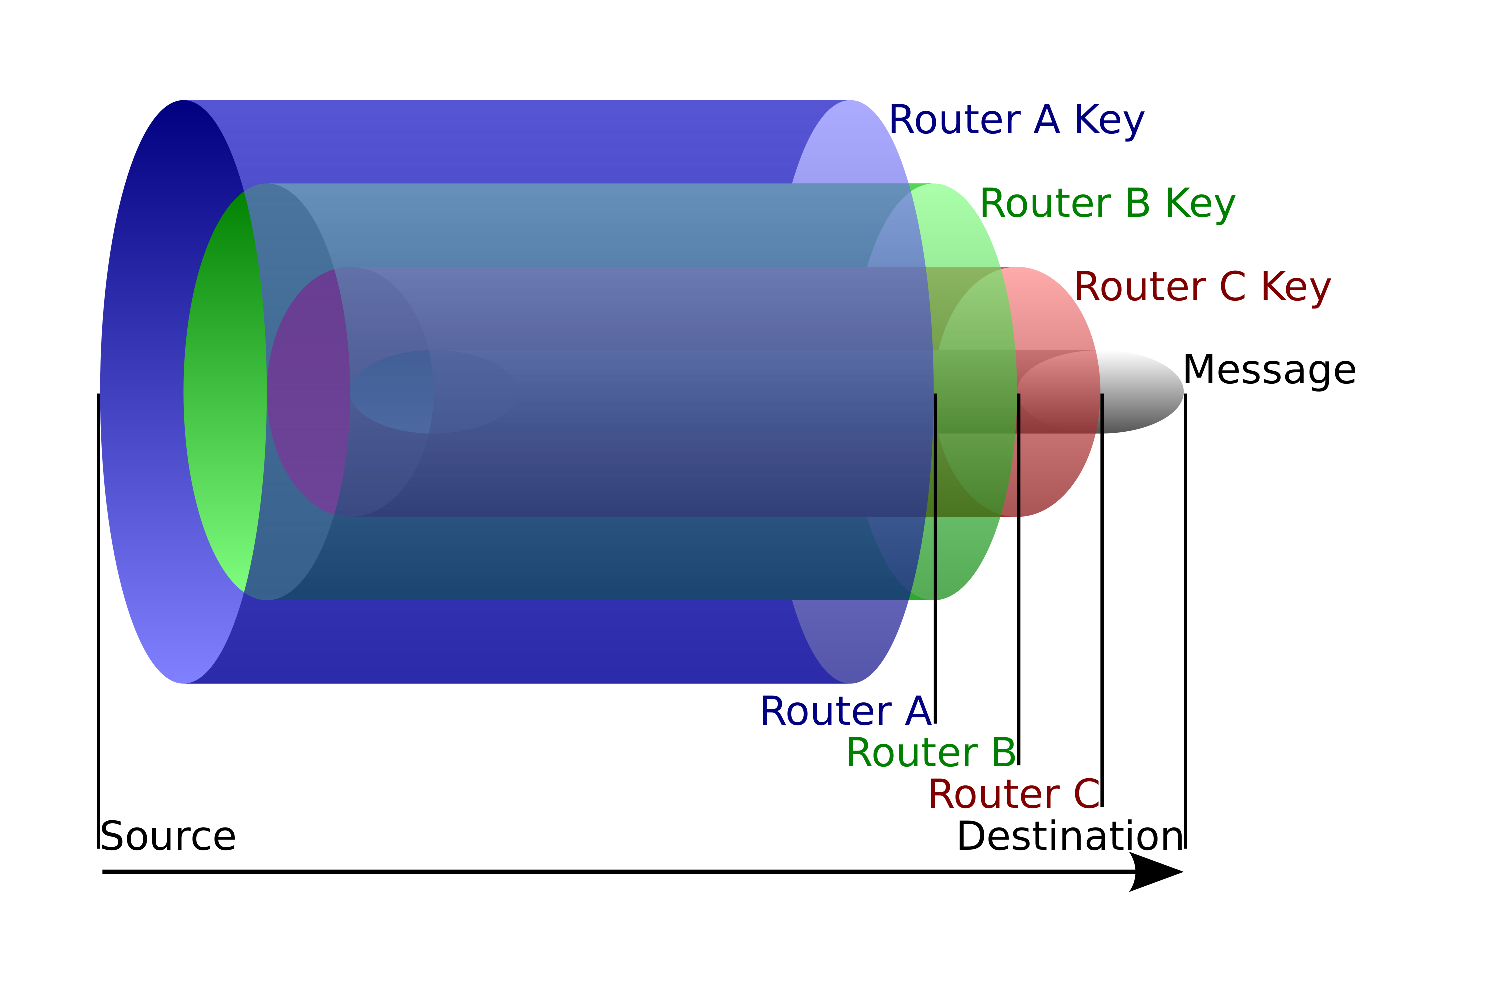
\includegraphics[scale=0.35]{imgs/onion}
  \caption{Onion routing graphical example of how layering works.}
  \label{fig:dtn-example}
\end{figure}

An example can be seen in figure \ref{fig:dtn-example} where the source node wants to send an anonymous message to a destination, using a previously chosen path composed by the nodes A, B and C. The source ciphers the message with the public key of C, B and A respectively. When the message reaches every hop, each node removes the external layer using the node private key.

In order to use onion routing a prior key exchange process needs to be performed. We consider that the loading of the network information behaviour as well as the keys sharing process will be done simultaneously at a previous stage, i.e: before starting the periodical routing. For example, in public transport networks the data as well as the needed keys will be shared before the scheduled route starts.

\subsection{Contact data representation}

% \red{Aim of this section: Explain how we stored the contact information of the network. Explain that we used a dynamic graph, defining what a graph is and what means to mean a dynamic one.} \\

Is it clear that we need to use a structure to represent the network activity. One method that seems to work is to use a graph structure as a way to represent network activity \red{\cite{a} \cite{b} \cite{c}}. Where each node of the network is represented as graph vertices and each contact between nodes as graph edges. 

A graph $G = (V, E)$ consists of two sets $V$ and $E$ \cite{gross2013handbook}. The elements of V are called \textit{vertices} or \textit{nodes} while the elements of E are called \textit{edges}. Each edge is composed by two vertices. Edges and vertices can have \textit{attributes}. An attribute is a value associated either to edges and vertices that permits to store information.

There is a subset of graphs in the graph theory called \textit{dynamic graphs}. Dynamic graphs permit to represent the evolution of the network during the time easily, i.e: nodes and edges may change positions and appear and/or disappear through time. To do so, we can set a pair of attributes that point out when a node appears and disappears.

Dynamic graph provides a good way to store information about the network. In our case this information will be related to contacts like the instant of time when the connection opportunity occurs and how long this contact has been.

In figure \ref{fig:dynamic-graph-example} the evolution of a given graph representing different contacts between buses in a public transport network is shown. In this example we can see that at the beginning, no contacts have been produced yet. As the time passes, the contacts (\textit{edges}) appear and disappear between buses (\textit{nodes}). 

\begin{figure}[h!tb]
\centering
  \subfloat[Full graph]{%
  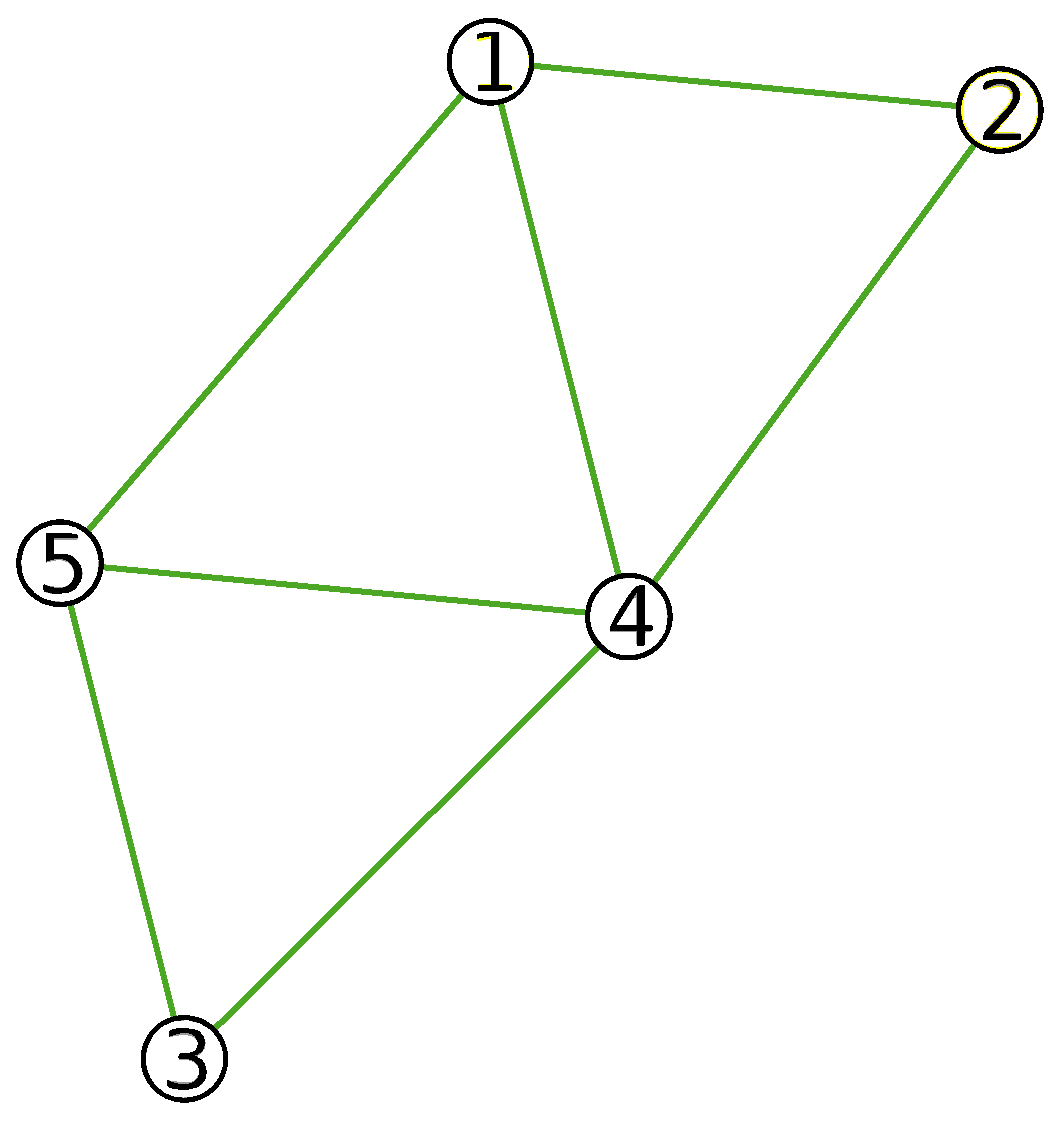
\includegraphics[scale=0.23]{imgs/example-dynamic/full}} \hfill
    \subfloat[$t = 0$]{%
    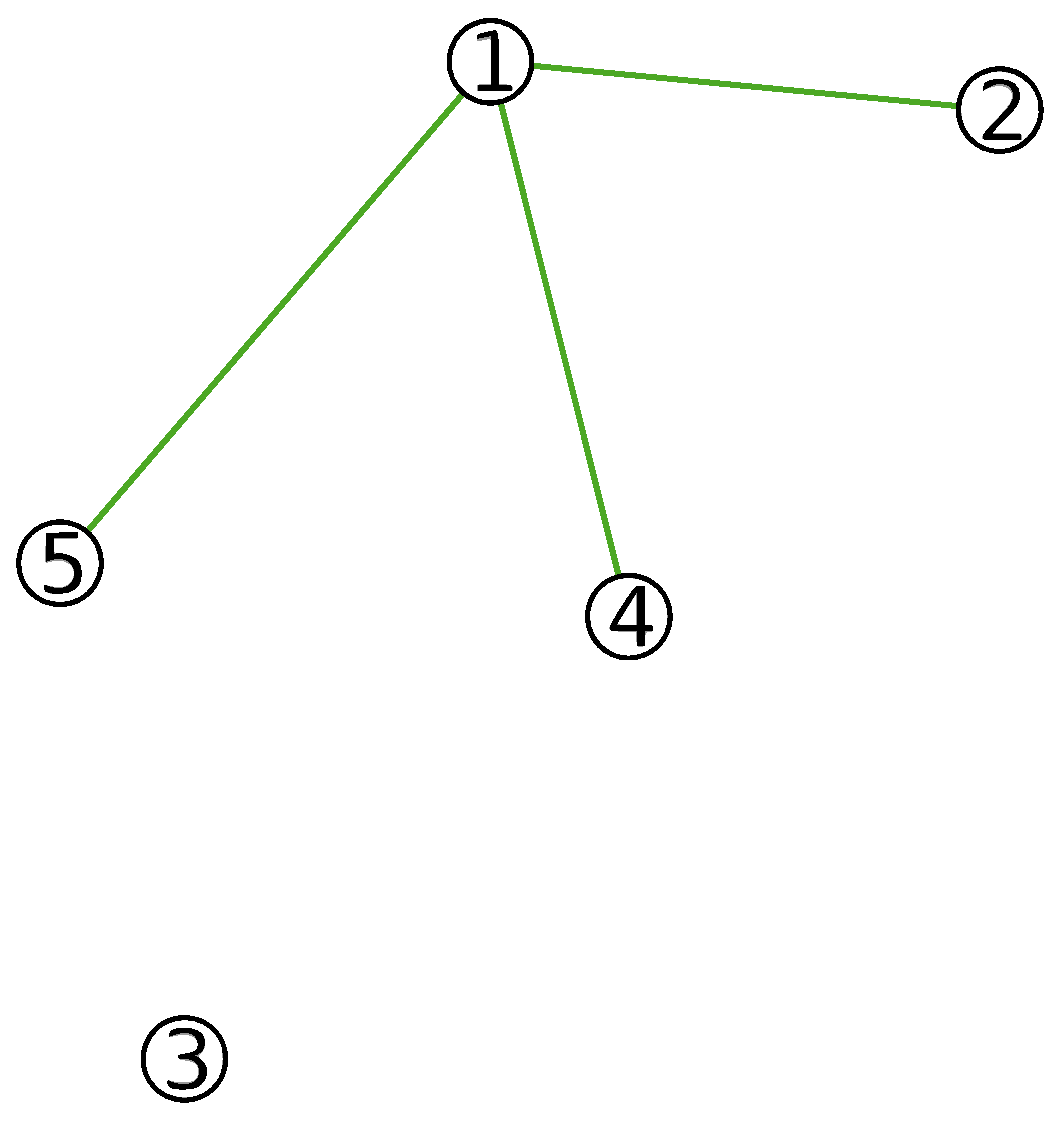
\includegraphics[width=.30\textwidth]{imgs/example-dynamic/t0}}\hfill
  \subfloat[$t = 1$]{%
    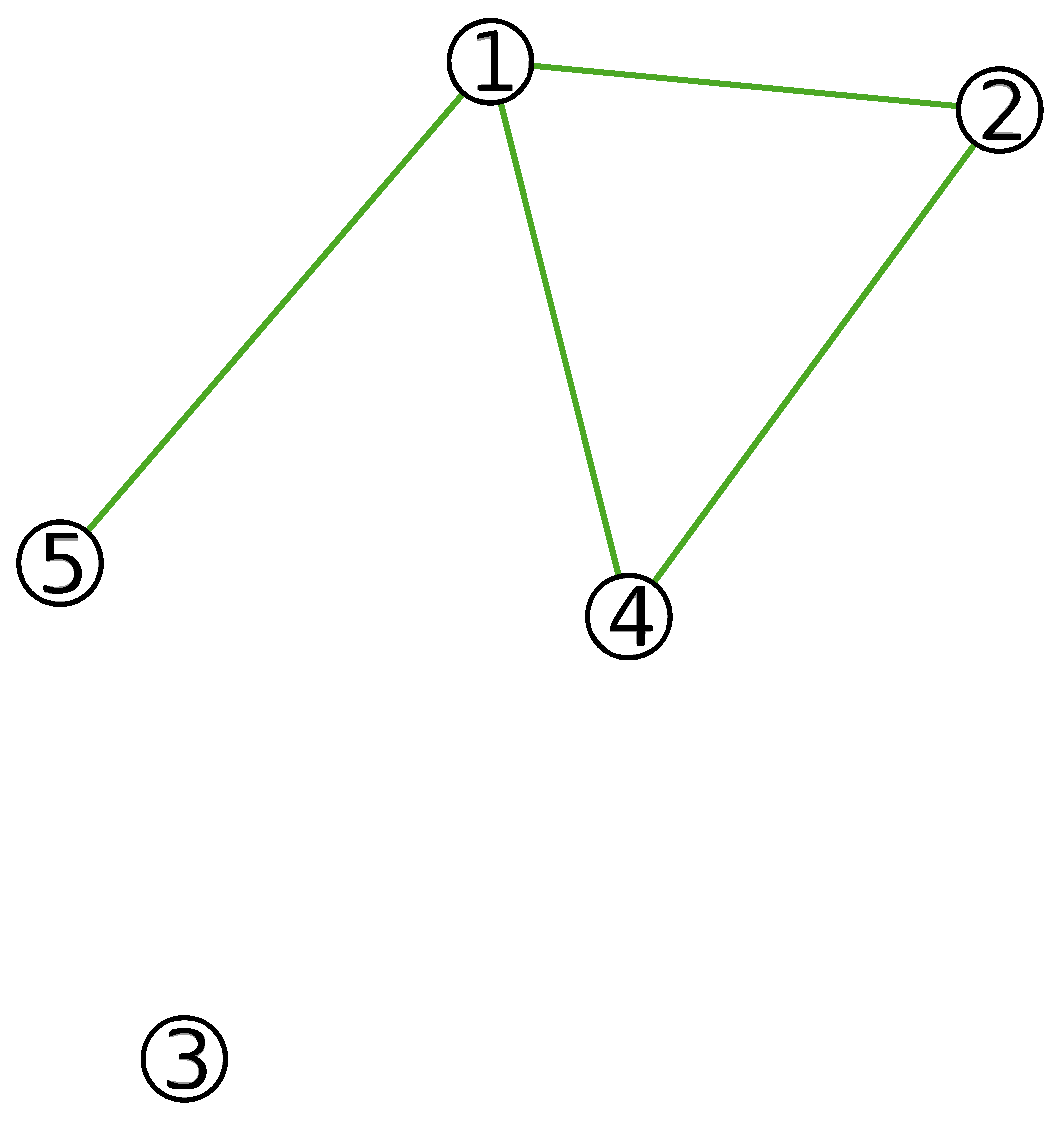
\includegraphics[width=.30\textwidth]{imgs/example-dynamic/t1}}\hfill
    \subfloat[$t = 2$]{%
    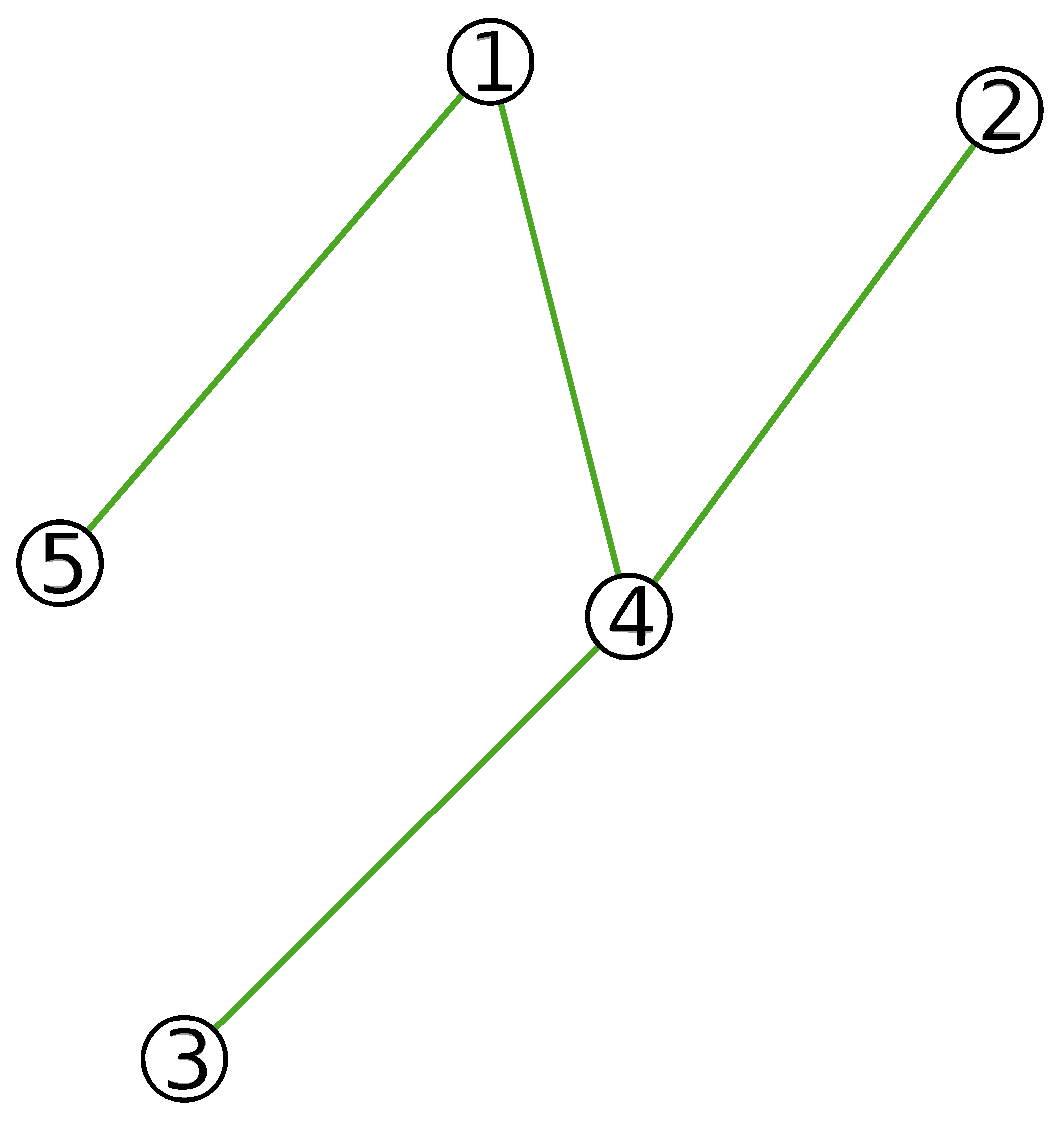
\includegraphics[width=.30\textwidth]{imgs/example-dynamic/t2}}\hfill
  \subfloat[$t = 3$]{%
    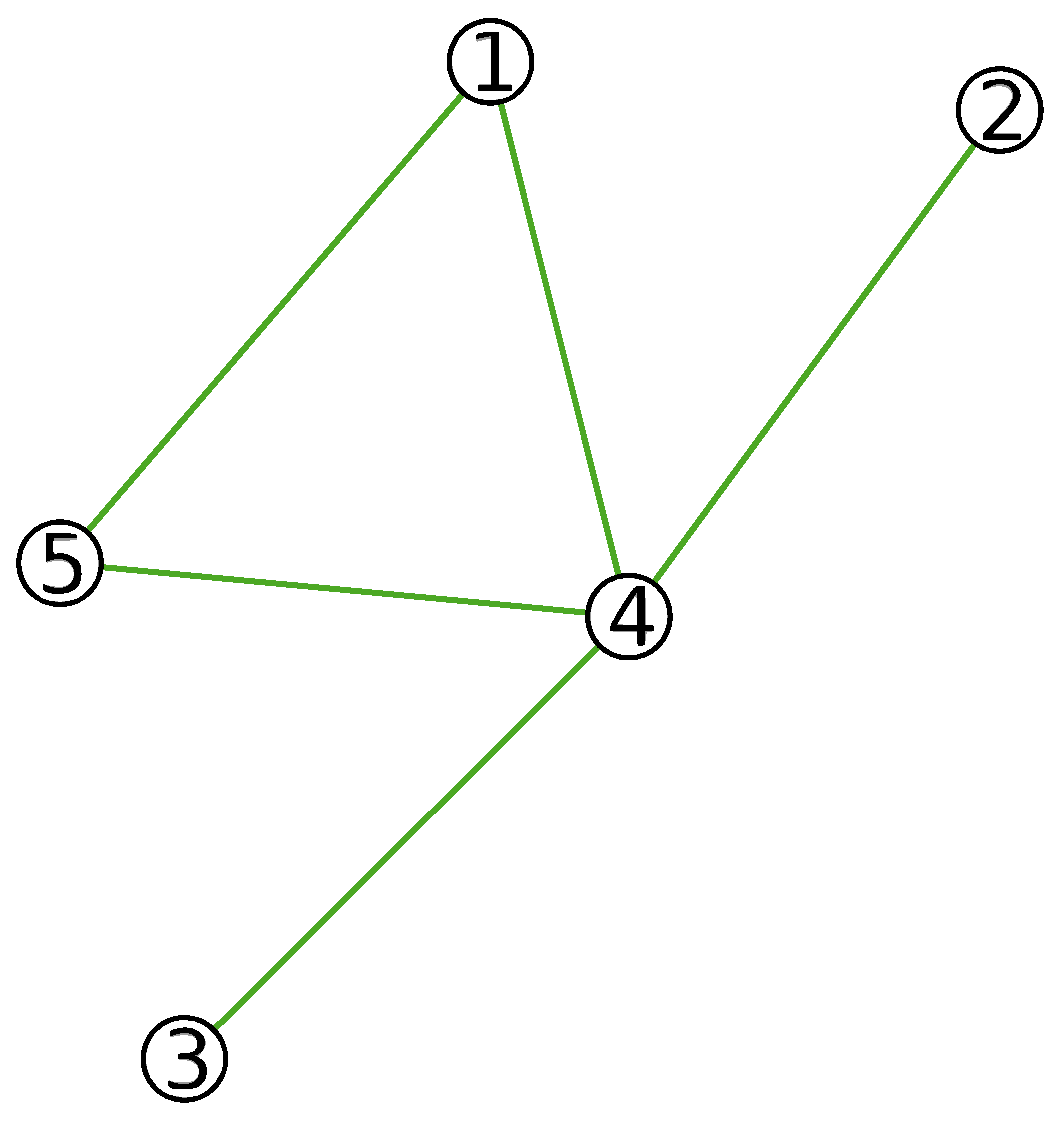
\includegraphics[width=.30\textwidth]{imgs/example-dynamic/t3}} \hfill
  \subfloat[$t = 4$]{%
    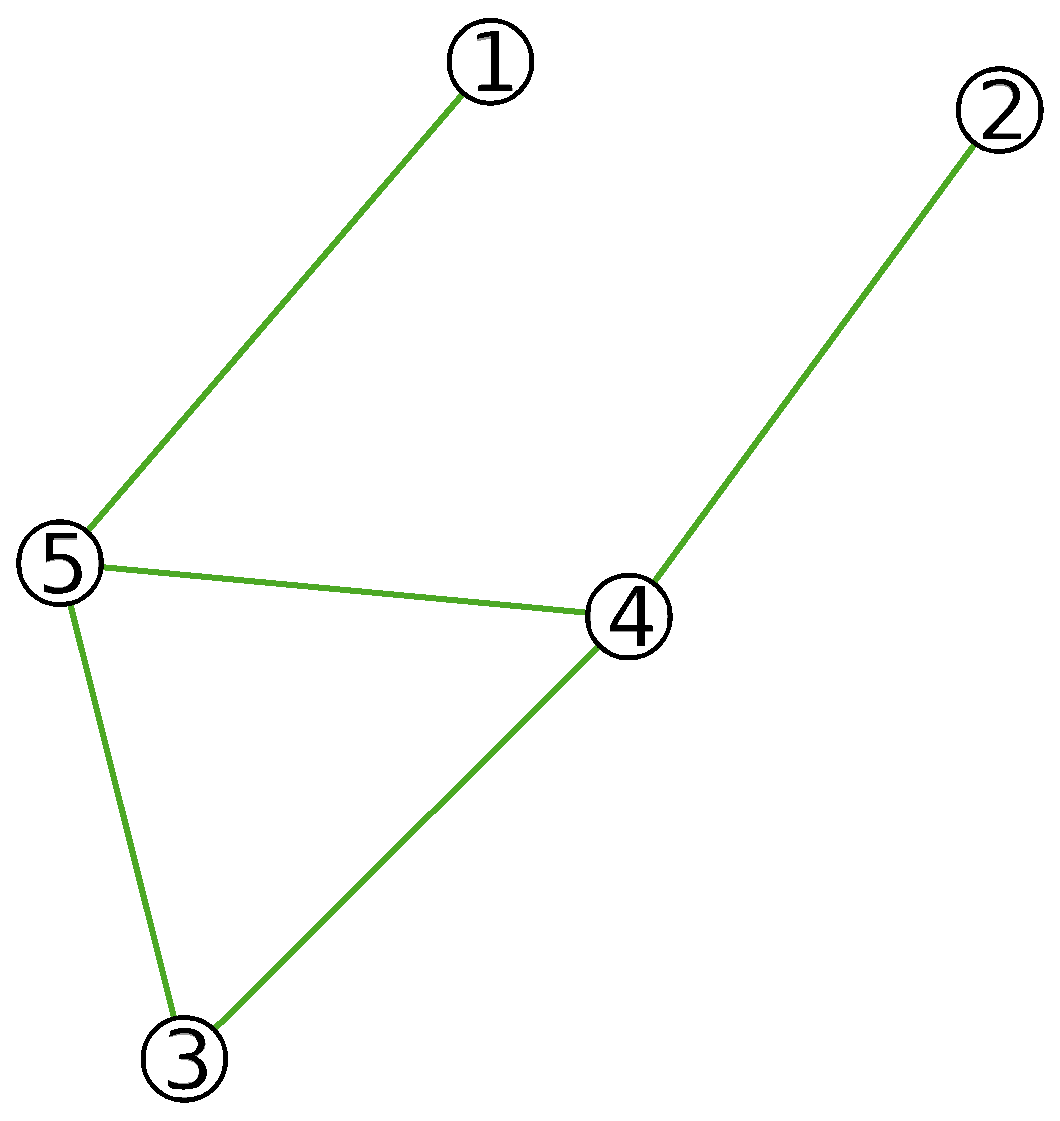
\includegraphics[width=.30\textwidth]{imgs/example-dynamic/t4}}\\
  \subfloat[$t = 5$]{%
    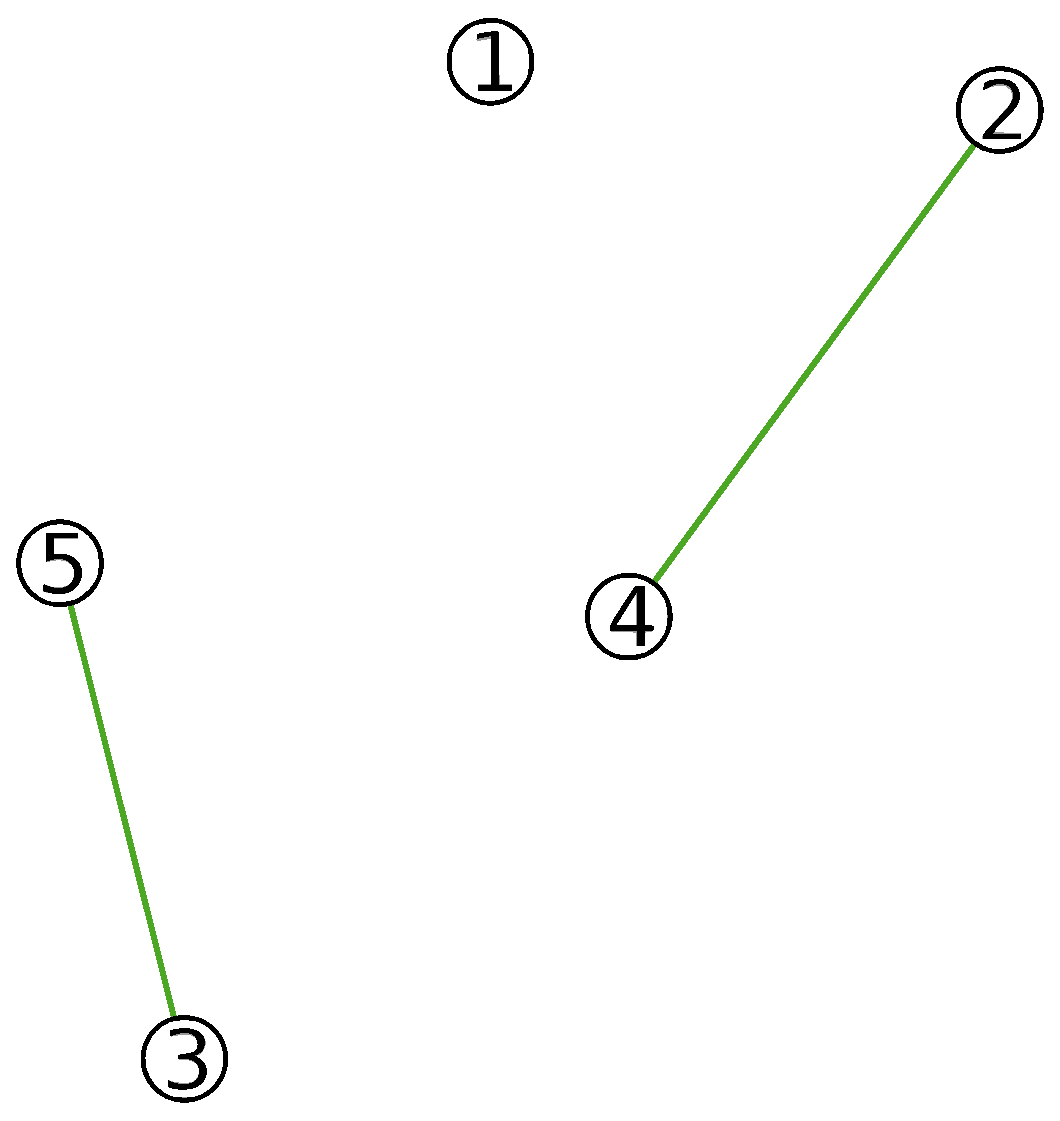
\includegraphics[width=.30\textwidth]{imgs/example-dynamic/t5}}\hfill
    \subfloat[$t = 6$]{%
    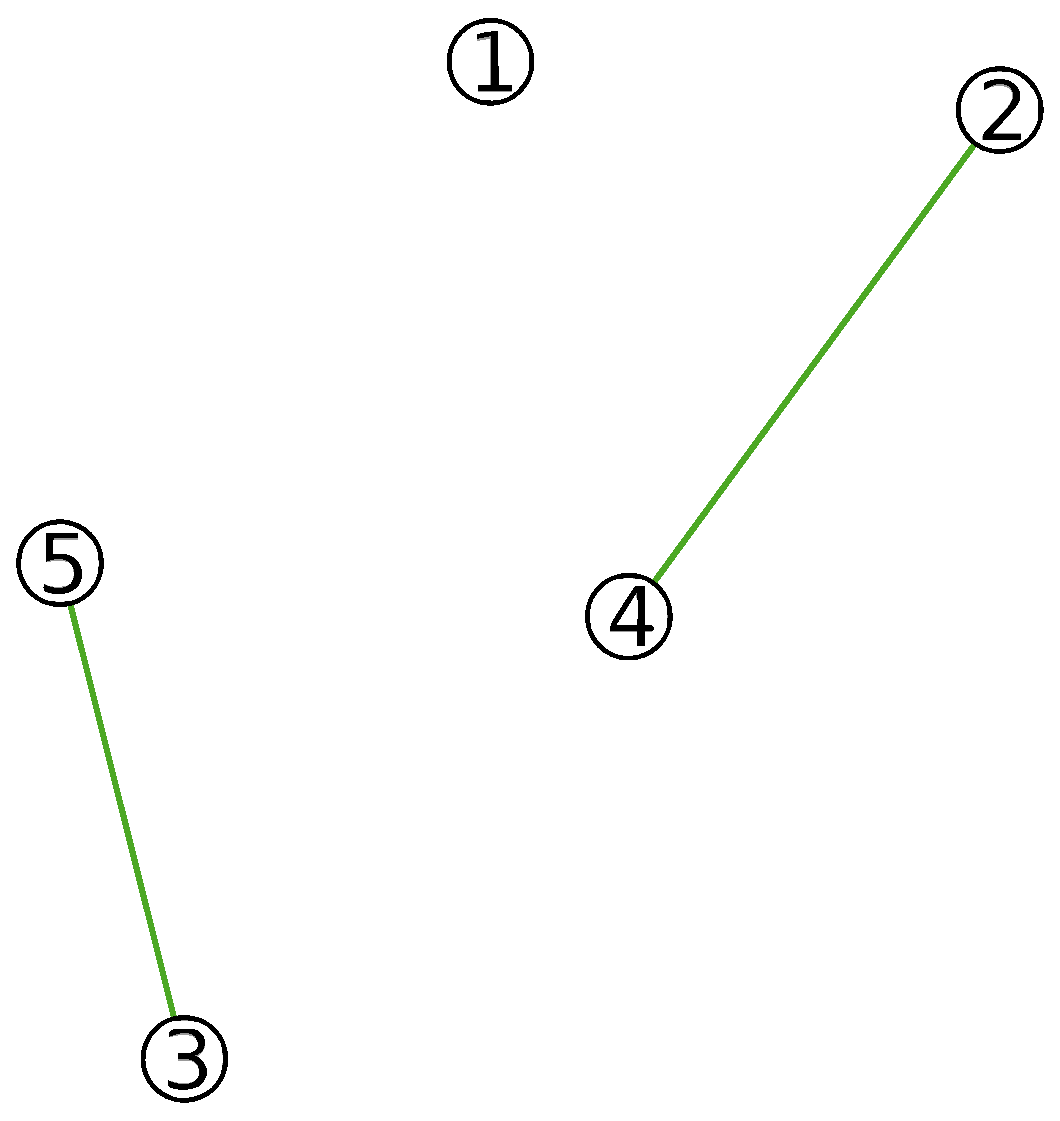
\includegraphics[width=.30\textwidth]{imgs/example-dynamic/t6}}\hfill
  \subfloat[$t = 7$]{%
    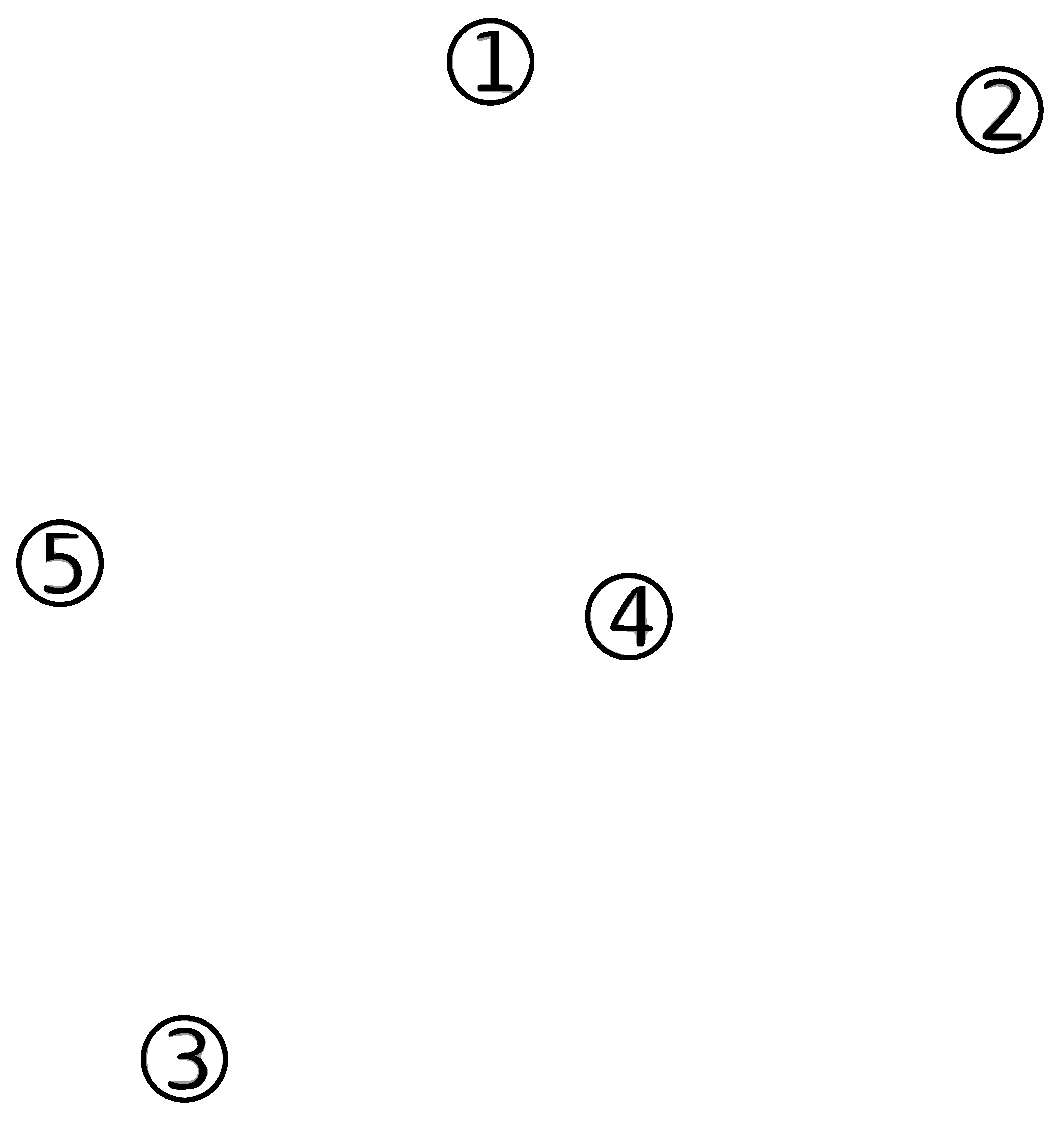
\includegraphics[width=.30\textwidth]{imgs/example-dynamic/t7}} 
  \caption{In $(a)$ the full (static) graph can be seen. In $(b)-(h)$ different snapshots in given instants of time showing the evolution of the dynamic graph are depicted.}
  \label{fig:dynamic-graph-example}
\end{figure}

\subsection{Path choosing}

%\red{Aim of this section: Explain what we did to get some useful paths according to a set of given parameters. Is important to explain the dynamic graph part, the algorithm itself, etc. \textbf{All theoretically!}} \\

Imagine we have a source node \textit{s} willing to send a message to a destination \textit{d} at time \textit{t} using onion routing. In onion routing you need to choose the number of nodes  \textit{n} where the message will pass through. Node \textit{s} obtains a path to perform the layering process and send the message. The time required to exchange the message between nodes is defined as \textit{tt}. 

To make even harder the path guessing for thirds, as the network knowledge is shared among all nodes, the node \textit{s} obtains a set of paths \textit{k} in order to choose one randomly. To sum up, we need a method \textit{f(s, d, t, n, k, tt)} that will retrieve a set of paths to finally choose one following the \textit{t}, \textit{n}, \textit{k} and \textit{tt} requirements. 

The procedures shown in Algorithm~\ref{alg:get-neighbors} and Algorithm~\ref{alg:get-paths} are an example of deterministic choosing for onion routing. Both of them inherit values to filter out unneeded paths. Specifically, in Algorithm~\ref{alg:get-neighbors} we return from a given node \textit{host} at time \textit{currentTime} a set of neighbors  that are available or will be available to forward the message. In Algorithm~\ref{alg:get-paths} we performed a recursive search to get up to \textit{k} paths of length \textit{n} from \textit{source} to \textit{destination}.

In figure~\ref{fig:dynamic-graph-example} we showed an example of contact data representation using dynamic graphs. Applying our path choosing method with: source node \textit{s=1}, destination node \textit{d=5}, starting time \textit{t=0}, number of paths \textit{k=4}, number of nodes of each path of \textit{n=5} and transmission time  \textit{tt=1}, we get the following paths: \\

\noindent\fbox{%
    \parbox{\textwidth}{%
        \textit{Path: 0} \\
		(1:0) $\rightarrow$ (2:0) $\rightarrow$ (4:1) $\rightarrow$ (1:2) $\rightarrow$ (5:3). Arrival time: 4\\
		\textit{Path: 1}\\
		(1:0) $\rightarrow$ (2:0) $\rightarrow$ (4:1) $\rightarrow$ (3:2) $\rightarrow$ (5:4). Arrival time: 5\\
		\textit{Path: 2}\\
		(1:0) $\rightarrow$ (4:0) $\rightarrow$ (1:1) $\rightarrow$ (4:2) $\rightarrow$ (5:3). Arrival time: 4\\
		\textit{Path: 3}\\
		(1:0) $\rightarrow$ (4:0) $\rightarrow$ (2:1) $\rightarrow$ (4:2) $\rightarrow$ (5:3). Arrival time: 4\\
		
		(n: t): Means message sent to node n at time t.
    }%
}

So we got 4 different paths composed by 5 nodes each (3 layers will be done). From the given set of paths, the source node \textit{s} will need to choose one in order to perform the onion routing itself.

\begin{algorithm}
\caption{Procedure to get valid neighbors of a given node}
\label{alg:get-neighbors}
\begin{algorithmic}[1]
\INHERIT (1) \textit{source}, source node. (2) \textit{destination}, destination node. (3) \textit{t}, when the message will be sent. (4) \textit{k}, maximum number of paths. (5) \textit{n}, number of nodes for each path (including source and destination). (6) \textit{tt}, transmission time required to forward the message.
\INPUT (1) \textit{host}, host node. (2) \textit{currentTime}, current time.
\OUTPUT (1) \textit{validNeighbors}, a set of valid neighbors to whom forward the message.
\Procedure{GetAvailableNeighbors }{host, currentTime}
\ForAll{$\textit{nbr} \in \textit{host.neighbors()}$} 
	\If{$(\textit{nbr}.activationTime + \textit{nbr}.contactDuration - \textit{tt}) \geq \textit{currentTime}$}
		\State $\textit{validNeighbors}.add(\textit{nbr})$
	\EndIf
\EndFor
\State \Return $\textit{validNeighbors}$
\EndProcedure
\end{algorithmic}
\end{algorithm}

\begin{algorithm}
\caption{Procedure to get paths that follows the inherited requirements}
\label{alg:get-paths}
\begin{algorithmic}[1]
\INHERIT (1) \textit{source}, source node. (2) \textit{destination}, destination node. (3) \textit{t}, when the message will be sent. (4) \textit{k}, maximum number of paths. (5) \textit{n}, number of nodes for each path (including source and destination). (6) \textit{tt}, transmission time required to forward the message.
\INPUT (1) \textit{currentPath}, current path. (2) \textit{currentTime}, current time.
\OUTPUT (1) \textit{paths}, a set of paths that follows the inherited requirements.
\Procedure{GetPaths}{currentPath, currentTime}

\If{$\textit{currentPath.size()} \neq \textit{n}$ and $\textit{paths.size()} < \textit{k}$}
	\State $\textit{node} \gets \textit{currentPath.last()}$
	\State $\textit{validNeighbors} \gets \textit{GetAvailableNeighbors(node, currentTime)}$
	\ForAll{$\textit{nbr} \in \textit{validNeighbors}$}
		\State $\textit{oldPath} \gets \textit{currentPath}$
		\State $\textit{nbr.sendingTime} \gets$ max$(\textit{nbr.activationTime}, \textit{currentTime}) + tt$
		\State $\textit{currentPath} \gets \textit{nbr}$
		\If{$\textit{nbr} = \textit{destination}$ and $\textit{currentPath.size()} = \textit{n}$ and $\textit{currentPath} \not\in \textit{paths}$}
			\State $\textit{validNeighbors}.add(\textit{nbr})$
		\Else
			\State \textsc{GetPaths}$(\textit{currentPath}, \textit{nbr.sendingTime})$	\Comment{Recursive part}
		\EndIf
		\State $\textit{currentPath} \gets \textit{oldPath}$
	\EndFor
\EndIf

\State \Return$\textit{paths}$
\EndProcedure
\end{algorithmic}
\end{algorithm}